\documentclass[conference]{IEEEtran}
\usepackage[T1]{fontenc}
\usepackage{amsmath}
\usepackage{amssymb}
\usepackage{amsthm}
\usepackage{graphicx}
\usepackage{booktabs}
\usepackage{array}
\usepackage{multirow}
\usepackage{cite}
\usepackage{xcolor}
\usepackage{hyperref}
\newtheorem{proposition}{Proposition}
\newtheorem{remark}{Remark}
\graphicspath{{figures/}}
\hypersetup{colorlinks=true, linkcolor=blue, citecolor=blue, urlcolor=blue}

\begin{document}

\title{Encoder-Side Task-Token Allocation for\\
       Multi-Task Wireless Semantic Communication}

\author{%
  \IEEEauthorblockN{Karl Khouri\textsuperscript{\dag} \quad Maria Slim\textsuperscript{\dag}}\\
  \IEEEauthorblockA{\textsuperscript{\dag}Department of Electrical and Computer Engineering,
                    American University of Beirut, Beirut, Lebanon}\\
  \IEEEauthorblockA{email: \texttt{kmk30@mail.aub.edu, mas194@mail.aub.edu}}%
}

\maketitle

% ============================================================
% ABSTRACT
% ============================================================
\begin{abstract}
We study how many channel symbols each task should receive when
several tasks are answered from the same transmitted sentence. Each
task owns a small set of learnable task tokens inside a FinBERT
encoder. A task token is mapped by a task-specific channel encoder to
four complex symbols, and only the first $k_t$ tokens of task $t$ are
transmitted. A small allocator chooses $k_t$ for every sentence from
a sentence summary, the average SNR reported by the receiver, the
channel type and an operator priority vector, under a cap on the
total number of task tokens and a price per symbol. Priority enters
the allocator through a nonnegative, context-dependent gain, which
makes each task's allocation score provably non-decreasing in its own
priority. On a cleaned Financial PhraseBank corpus with three tasks
(sentiment, forward-looking statements and ESG) over AWGN, Rayleigh
and Rician channels, SNR-adaptive allocation reaches the accuracy of
fixed splits with 17 to 30 percent fewer symbols and sends 12 instead
of 48 symbols per sentence on clean channels. With 32 task tokens per
task on AWGN, the allocator matches the accuracy of a fixed 16-token
split with 39 percent fewer symbols. The gain-based priority input
raises the accuracy of the prioritized task by 1.8 points, against
0.4 points for a conventional priority embedding. An input ablation
shows that the SNR input is essential, the priority input is useful
and the sentence summary adds a small but significant gain. A lookup
table that applies greedy marginal allocation to average validation
loss curves performs on par with the learned allocator.
\end{abstract}

\begin{IEEEkeywords}
Semantic communication, multi-task learning, resource allocation,
task tokens, adaptive rate, FinBERT.
\end{IEEEkeywords}

% ============================================================
% I. INTRODUCTION
% ============================================================
\section{Introduction}
\label{sec:intro}

Semantic communication transmits the meaning of a source rather than
its raw bits, with the aim of reducing the number of channel uses
while preserving the performance of downstream tasks
\cite{gunduz2023beyond}. Learned transceivers such as DeepSC
\cite{xie2021deepsc} and its multi-task extensions
\cite{sheng2024multitask} train the semantic encoder, the channel
code and the task heads jointly. When several tasks are answered from
the same sentence, a practical question follows: how many channel
symbols does each task need, for this sentence, on this channel and
under this operator priority?

Our earlier study of this question allocated a shared decoded
representation after the channel with soft per-task masks. That
design did not deliver reliable gains: only a hard equal split
improved consistently across channels, and doubling the channel rate
without controlling the allocation reduced accuracy. We take two
lessons from it. First, allocation should happen before the channel,
in units that belong to a single task, so that a task's information
is already separated when the symbols are sent. Second, more symbols
are not automatically better, so the number of symbols sent should
itself be a decision.

This paper implements both lessons. Each task owns learnable task
tokens inside the encoder. The transmitter sends only the first $k_t$
tokens of task $t$, and a small allocator chooses the counts
$(k_1, \ldots, k_T)$ for every sentence from the sentence, the
average SNR, the channel type and the operator priority, under a
total cap and a price per symbol.

\subsection{Contributions}

\begin{enumerate}
  \item An encoder-side multi-task architecture in which each task
        owns ordered task tokens with restricted attention, each
        token is coded into four complex symbols by a task-specific
        channel encoder, and the number of tokens per task is chosen
        before transmission.
  \item A learned allocator whose priority input enters through a
        nonnegative, context-dependent gain. This structure
        guarantees that a task's score never decreases when its own
        priority increases, and in our experiments it steers
        accuracy toward the prioritized task far more strongly than
        a priority embedding.
  \item An evaluation on a cleaned three-task financial corpus over
        AWGN, Rayleigh and Rician channels, with shared noise
        realizations, three seeds and paired-bootstrap confidence
        intervals. It covers per-task token saturation, fixed-cap
        redistribution, variable-rate operation, priority steering,
        larger token budgets, and an ablation of every allocator
        input against fixed splits and a greedy lookup table.
\end{enumerate}

% ============================================================
% II. SYSTEM MODEL
% ============================================================
\section{System Model}
\label{sec:system}

Fig.~\ref{fig:arch} shows the end-to-end pipeline. A sentence $x$ is
answered for $T{=}3$ tasks: Sentiment (3 classes), forward-looking
statement detection, FLS (3 classes), and ESG (4 classes: environmental,
social, governance, none).

\begin{figure*}[t]
  \centering
  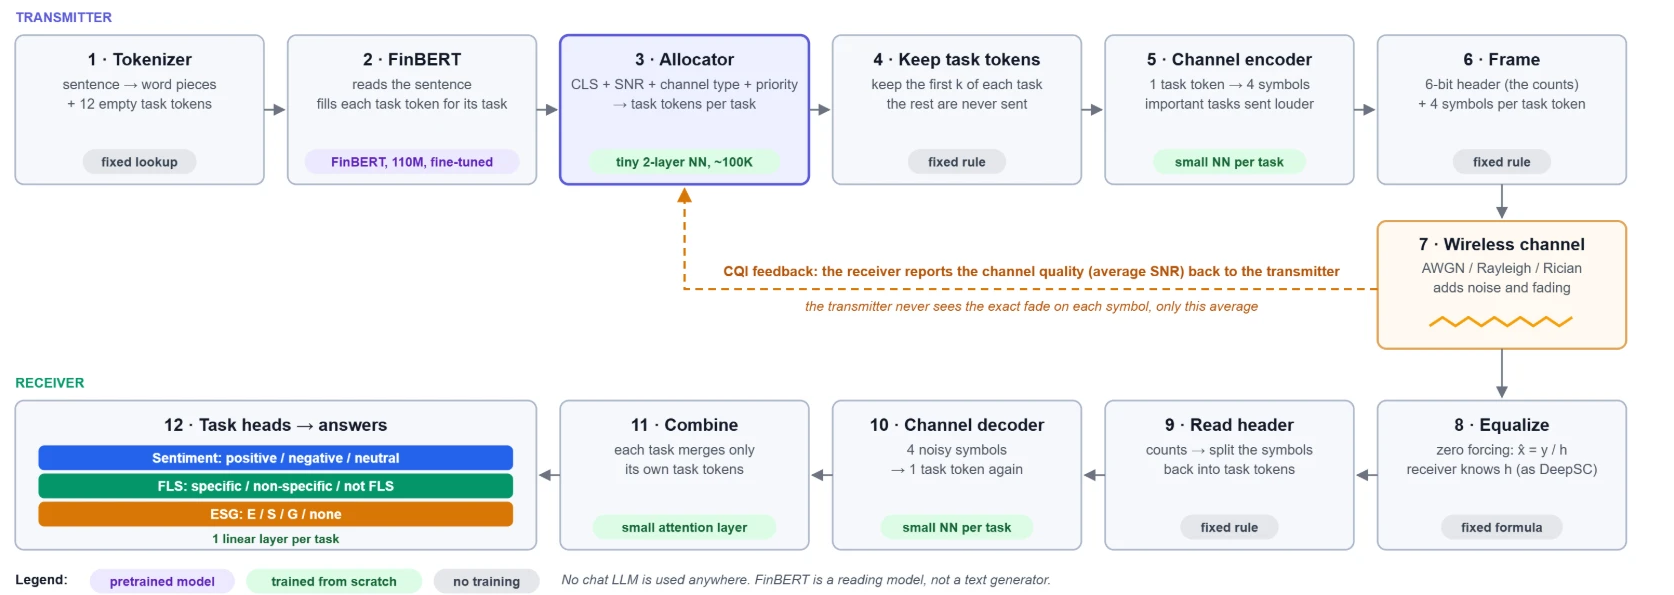
\includegraphics[width=\textwidth]{architecture.png}
  \caption{End-to-end pipeline. The transmitter encodes the sentence
           with task tokens, the allocator chooses how many task
           tokens each task sends, and each kept token is coded into
           four complex symbols. The receiver equalizes, splits the
           symbols by task using the header, decodes each token and
           pools each task's tokens before its head. Per-task power
           scaling (step 5) was disabled in all experiments, so every
           kept token is sent at the same average power.}
  \label{fig:arch}
\end{figure*}

\subsection{Task Tokens and Encoder}

Each task owns $J$ learnable task-token vectors (``slots''), giving
$TJ$ slots in total. The encoder input is
\texttt{[CLS]}, the $TJ$ task tokens, then the word pieces of the
sentence. Attention is restricted as follows: a task token attends to
the words and to the tokens of its own task; words, \texttt{[CLS]}
and \texttt{[SEP]} attend only to words. Words therefore never see the
task tokens, which keeps word processing identical to the pretrained
encoder, and tokens of different tasks never exchange information.
The encoder is FinBERT \cite{yang2020finbertfls}
(\texttt{finbert-pretrain}, 110M parameters, hidden size $d{=}768$).
We keep the \texttt{[CLS]} output as a sentence summary and the $TJ$
task-token outputs; word outputs are discarded.

\subsection{Token Selection and Channel Coding}

Given counts $k_t \in \{1, \ldots, J\}$, the transmitter keeps the
first $k_t$ tokens of task $t$; the remaining tokens are never sent.
A task-specific channel encoder ($768 \to 256 \to 8$ reals, ReLU)
maps each kept token to $L{=}4$ complex symbols, normalized to unit
average energy per symbol. A sentence therefore uses
$N = 4 \sum_t k_t$ channel uses. A short header carries the counts and
is assumed error-free.

\subsection{Channel and Receiver}

The channel is $y = h x + n$ with $n \sim \mathcal{CN}(0, \sigma^2)$
and $\sigma^2 = 10^{-\mathrm{SNR}/10}$, with fading drawn
independently per symbol. AWGN uses $h{=}1$, Rayleigh uses
$h \sim \mathcal{CN}(0,1)$, and Rician uses
$h = \sqrt{K/(K{+}1)}\,e^{j\theta} + \sqrt{1/(K{+}1)}\,\mathcal{CN}(0,1)$
with $K{=}4$; all three satisfy $\mathbb{E}|h|^2 = 1$. The receiver
knows $h$ and applies zero forcing, $\hat{x} = y/h$, as in DeepSC
\cite{xie2021deepsc}. On AWGN zero forcing reduces to the identity.
The header splits the received symbols back into task tokens. A
task-specific channel decoder ($8 \to 256 \to 768$) restores each
token, a per-task attention pooling layer with a learned query merges
the received tokens of that task (unsent slots are excluded), and one
linear head per task produces the prediction.

\subsection{Channel Quality Feedback}

The receiver reports the average SNR to the transmitter (CQI). The
allocator uses this average and the channel type but never the
per-symbol fading coefficients. In simulation the reported SNR equals
the true SNR of the sentence.

% ============================================================
% III. ALLOCATION
% ============================================================
\section{Token Allocation}
\label{sec:alloc}

\subsection{Problem}

For priorities $\mathbf{w} = (w_1, \ldots, w_T)$ with $w_t \geq 0$
and $\sum_t w_t = 1$, a total cap $K$ and a per-task maximum $J_{\max}$,
the allocator chooses integer counts to minimize
\begin{equation}
  \mathbb{E}\Big[\sum_{t=1}^{T} w_t\, \mathrm{CE}_t(k_t)
              + \lambda \sum_{t=1}^{T} k_t\Big]
  \quad \text{s.t.} \quad
  1 \leq k_t \leq J_{\max}, \;\; \sum_t k_t \leq K,
  \label{eq:problem}
\end{equation}
where $\mathrm{CE}_t(k_t)$ is the cross-entropy of task $t$ when it
sends $k_t$ tokens and $\lambda \geq 0$ is a price per task token.
With $\lambda{=}0$ the allocator only redistributes tokens under the
cap; with $\lambda{>}0$ it may send fewer tokens than the cap allows.
The cap is an external resource limit and is not learned.

\subsection{Greedy Marginal Allocation}

When each $\mathrm{CE}_t$ has diminishing returns in $k_t$, the
classical marginal-analysis argument of Fox \cite{fox1966marginal}
gives the optimum of (\ref{eq:problem}): start from one token per
task and repeatedly give the next token to the task with the largest
priority-weighted loss reduction
$w_t\,[\mathrm{CE}_t(k_t) - \mathrm{CE}_t(k_t{+}1)]$, stopping when this
reduction does not exceed $\lambda$ or when a limit is reached. This
is the discrete counterpart of a marginal-equalization condition: at
the optimum, every task with an interior allocation has the same
priority-weighted marginal return, and $\lambda$ plays the role of
the Lagrange multiplier of the symbol budget. We use this rule in two
ways: applied to measured average curves it defines a lookup-table
baseline (\S\ref{ssec:table}), and applied to each test sentence's own
losses it defines a hindsight oracle.

\subsection{Learned Allocator}

The allocator receives the \texttt{[CLS]} output (768 values), the SNR
in dB divided by 10 and expanded by a linear layer with ReLU to 32
values, the channel type as a one-hot vector expanded to 32 values,
and the priority vector $\mathbf{w}$. Optionally it also receives a
confidence input: for each task, the normalized entropy of that
task's head when all its tokens pass a noise-free channel, computed
at the transmitter and excluded from gradient flow. The concatenated
context passes through one hidden layer of 128 ReLU units, giving a
representation $\mathbf{u}$, and two linear heads produce a base score
$b_t(\mathbf{u})$ and a raw gain $g_t(\mathbf{u})$ for each task. The
score of task $t$ is
\begin{equation}
  s_t = b_t(\mathbf{u}) + \mathrm{softplus}\big(g_t(\mathbf{u})\big)\, w_t .
  \label{eq:score}
\end{equation}
The base score expresses how many tokens the task needs for this
sentence and channel; the gain expresses how much the operator's
priority should count in this situation. The priority does not enter
the hidden layer.

\begin{proposition}
\label{prop:monotone}
For any sentence, SNR, channel type and network weights, the score
$s_t$ in (\ref{eq:score}) is non-decreasing in the task's own priority
$w_t$.
\end{proposition}
\begin{proof}
$\mathbf{u}$ does not depend on $\mathbf{w}$, so
$\partial s_t / \partial w_t = \mathrm{softplus}(g_t(\mathbf{u})) \geq 0$.
\end{proof}

This form is a varying-coefficient model \cite{hastie1993varying}: the
score is affine in $w_t$ with an intercept and a slope that depend on
the context, as in networks that generate their own coefficients
\cite{alvarezmelis2018senn}. The sign constraint through softplus
follows the use of softplus to enforce shape constraints
\cite{dugas2001softplus}, and the guarantee is an instance of partial
monotonicity \cite{sill1998monotonic, daniels2010monotone}. A
conventional design that embeds $\mathbf{w}$ into the hidden layer
offers no such guarantee; we compare against it in
\S\ref{ssec:priority}.

The scores are turned into counts by fixed operations. Soft counts are
$c_t = 1 + (J_{\max} - 1)\,\sigma(s_t)$. If $\sum_t c_t > K$, the part
above one token is scaled down,
$c_t \leftarrow 1 + (c_t - 1)(K - T)/(\sum_j c_j - T)$. The counts are
rounded to the nearest integer; if rounding exceeds the cap, all
counts are rounded down and the remaining tokens go to the largest
fractional parts, with ties broken by priority. The output layers are
initialized to zero and the gain bias to $-5$, so training starts from
an almost equal split for any priority.

Rounding has no useful gradient, so training uses a straight-through
estimator \cite{bengio2013estimating}: the forward pass uses the hard
counts and the hard token masks, while the backward pass uses the soft
counts and soft masks
$m_{t,j} = \sigma\big((c_t - j + 0.5)/\tau\big)$ with $\tau = 0.3$.
The allocator is trained with random priorities
$\mathbf{w} \sim \mathrm{Dir}(1,1,1)$ drawn per batch, so a single
model serves every priority at run time, as in loss-conditional
training \cite{dosovitskiy2020yoto, navon2021pareto}.

\subsection{SNR Lookup Table}
\label{ssec:table}

The lookup table uses no learning. On the validation sentences, every
task is sent with $k = 1, \ldots, J_{\max}$ tokens at every evaluation
SNR on every channel, and the cross-entropy is averaged over sentences
and channels. At run time the table takes the SNR and the priority
vector and applies the greedy rule above to these average curves
under the same cap, per-task maximum and price $\lambda$. Every
sentence with the same SNR and priority receives the same counts.

% ============================================================
% IV. EXPERIMENTAL SETUP
% ============================================================
\section{Experimental Setup}
\label{sec:setup}

\subsection{Data}

We use the Financial PhraseBank \cite{malo2014phrasebank}
(\texttt{Sentences\_50Agree}, 4,846 sentences) with its human
sentiment labels. FLS and ESG labels are produced by the FinBERT-FLS
and FinBERT-ESG classifiers \cite{huang2023finbert}, so these two tasks
carry a label-noise floor. We repair 111 sentences whose accented
characters were corrupted by a character-encoding error, drop exact
duplicates (keeping one copy when labels agree and none when they
conflict), drop near-duplicates that differ only in numbers and carry
conflicting sentiment labels, and drop four fragments of fewer than
four tokens. The resulting corpus has 4,825 sentences. Class counts
are 600/2,865/1,360 for negative/neutral/positive sentiment,
3,715/92/1,018 for not-FLS/non-specific/specific FLS, and
299/893/53/3,580 for environmental/social/governance/none ESG.

The corpus is split 70/10/20 into 3,379 training, 480 validation and
966 test sentences. The split is stratified by the joint label of the
three tasks, and sentences that differ only in numbers are kept in
the same split so that no template appears in both training and test.
The same split is used by every run.

\subsection{Training}

Training has two stages. In the first stage, the encoder, task tokens,
channel encoders and decoders, pooling layers and heads are trained
for 12 epochs with nested dropout \cite{rippel2014nested}: for every
sentence and task, a cut-off $j$ is drawn uniformly from
$\{1, \ldots, J\}$ and only the first $j$ tokens are sent, which
teaches the first token to carry the most information. The channel
type is drawn per batch and the SNR per sentence, uniformly in
$[-10, 10]$\,dB. The loss is the sum of the three cross-entropies,
with inverse-frequency class weights on FLS and ESG computed on the
training split and scaled to an average weight of one, so that no
task's loss is shrunk relative to another. We use AdamW with learning
rate $2{\times}10^{-5}$ for the encoder and $10^{-3}$ elsewhere,
batch size 16, and keep the epoch with the lowest validation loss.

In the second stage, the pipeline is frozen, the encoder outputs are
computed once, and only the allocator is trained for 30 epochs
(AdamW, learning rate $10^{-3}$, batch size 16) on
(\ref{eq:problem}) with random channel, SNR and priority. After every
epoch the same objective, including $\lambda$ times the number of
tokens, is evaluated on the validation split with fixed noise and
equal priority, and the best epoch is kept. We also trained the
allocator jointly with the pipeline in a single stage; the outcome is
reported in \S\ref{ssec:fixedcap}.

\subsection{Evaluation}

Test SNRs are $\{-15, -10, -5, -2, 0, 2, 5, 10, 15, 20\}$\,dB. For each
test batch, channel and SNR, one fading and noise realization is drawn
from a fixed seed and shared by every method, so all methods face the
same channel. Every configuration is trained with three seeds.
Accuracy is reported per task and as the mean of the three tasks.
Confidence intervals are paired-bootstrap 95\% intervals with 10,000
resamples over (seed, channel, SNR, sentence) units. Baselines are
evaluated on the same frozen pipeline: fixed splits (no allocator),
equal split at the cap, proportional split $\mathrm{round}(K\mathbf{w})$,
a random split with the allocator's total, the SNR lookup table, and
the hindsight oracle, which uses the test labels and the realized
noise and is reported only as an upper bound.

Two token budgets are studied. In the main setting each task owns
$J{=}4$ tokens ($T J {=} 12$ slots, at most 48 symbols) on all three
channels. In the large-budget setting each task owns $J{=}32$ tokens
(96 slots), the per-task maximum is $J_{\max} = K/2$, training and
testing use AWGN only, and the channel-type input is removed.

% ============================================================
% V. RESULTS
% ============================================================
\section{Results}
\label{sec:results}

\subsection{Token Saturation}
\label{ssec:saturation}

Table~\ref{tab:saturation} reports the accuracy gained when every task
sends four tokens instead of one ($J{=}4$, no allocator). On noisy
channels each additional token helps, most for FLS and ESG. On clean
channels a single token per task already reaches the accuracy of four:
at 15\,dB the gain is below one point on every channel and task. The
channel ordering is as expected: AWGN is easiest, Rician intermediate
and Rayleigh hardest at every SNR. The accuracy ceilings at 15\,dB are
about 83 percent for Sentiment, 95 percent for FLS and 88 percent for
ESG.

\begin{table}[!htbp]
  \centering
  \caption{Accuracy gain (points) from 1 to 4 task tokens per task,
           $J{=}4$, no allocator, mean of 3 seeds.}
  \label{tab:saturation}
  \footnotesize
  \begin{tabular}{llccc}
    \toprule
    Channel & SNR (dB) & Sentiment & FLS & ESG \\
    \midrule
    \multirow{3}{*}{AWGN}     & $-5$ & $+8.5$  & $+12.5$ & $+13.6$ \\
                              & $5$  & $+0.2$  & $+0.0$  & $+0.6$ \\
                              & $15$ & $+0.0$  & $+0.0$  & $+0.6$ \\
    \midrule
    \multirow{3}{*}{Rician}   & $-5$ & $+10.0$ & $+14.0$ & $+14.8$ \\
                              & $5$  & $+0.8$  & $+0.6$  & $+1.0$ \\
                              & $15$ & $-0.1$  & $+0.1$  & $+0.6$ \\
    \midrule
    \multirow{3}{*}{Rayleigh} & $-5$ & $+12.5$ & $+18.4$ & $+18.2$ \\
                              & $5$  & $+3.3$  & $+3.3$  & $+5.1$ \\
                              & $15$ & $+0.3$  & $+0.6$  & $+0.7$ \\
    \bottomrule
  \end{tabular}
\end{table}

\subsection{Fixed Cap: Redistributing Eight Tokens}
\label{ssec:fixedcap}

With $J{=}4$, $K{=}8$ and $\lambda{=}0$, every method sends about 32
symbols and differs only in how the eight tokens are split
(Table~\ref{tab:cap8}). All deployable methods lie within 0.25
points of the equal split. The learned allocator gains $+0.07$ points over
the equal split on average (per seed $+0.04$, $+0.20$, $-0.04$), and
with the confidence input $+0.19$ points with the same sign on every
seed ($+0.18$, $+0.17$, $+0.21$). The allocators move accuracy from
Sentiment to ESG, where additional tokens help most.

\begin{table}[!htbp]
  \centering
  \caption{Fixed cap $K{=}8$, $J{=}4$, $\lambda{=}0$. Accuracy (\%)
           averaged over three channels, ten SNRs and three seeds.}
  \label{tab:cap8}
  \footnotesize
  \setlength{\tabcolsep}{3pt}
  \resizebox{\columnwidth}{!}{%
  \begin{tabular}{lccccc}
    \toprule
    Method & Symbols & Sent. & FLS & ESG & Mean \\
    \midrule
    Equal split 3/3/2 (no allocator) & 32.0 & 78.08 & 89.14 & 79.35 & 82.19 \\
    Proportional split               & 32.0 & 78.08 & 87.46 & 81.25 & 82.26 \\
    Random split                     & 31.9 & 77.32 & 88.27 & 80.27 & 81.95 \\
    SNR lookup table                 & 31.3 & 77.32 & 88.51 & 81.23 & 82.36 \\
    Learned allocator                & 31.9 & 77.80 & 88.02 & 80.95 & 82.26 \\
    Learned allocator + confidence   & 32.0 & 76.97 & 88.94 & 81.21 & 82.37 \\
    Learned allocator, priority embedding & 31.9 & 77.08 & 88.85 & 80.87 & 82.27 \\
    \midrule
    Hindsight oracle (not deployable) & 22.9 & 82.61 & 92.54 & 85.85 & 87.00 \\
    \bottomrule
  \end{tabular}%
  }
\end{table}

The room for redistribution at a fixed cap is small. Using the
measured per-task curves, the best fixed split chosen in hindsight
for each channel and SNR exceeds the equal split by at most 0.85
points (Rayleigh, $-5$\,dB) and by less than 0.3 points in most cases.
The much larger margin of the hindsight oracle comes from knowing each
sentence's labels and noise realization, which no transmitter can
know.

When the allocator was trained jointly with the pipeline in one
stage, it remained at its initial 3/3/2 split (mean accuracy 83.82
against 83.79 for the equal split): the pipeline began to overfit
after two allocator epochs, so the selected checkpoint came from a
point where the allocator had not yet moved. The two-stage schedule
of \S\ref{sec:setup} was adopted for this reason.

\subsection{Variable Rate}
\label{ssec:rate}

With $J{=}4$, $K{=}12$ (so the cap does not bind) and five prices
$\lambda \in \{0.001, 0.003, 0.01, 0.03, 0.1\}$, the allocator decides
the total number of tokens as well as the split.
Table~\ref{tab:rate} reports accuracy against symbols and
Table~\ref{tab:target} the number of symbols needed to reach a given
accuracy. SNR-adaptive allocation reaches the accuracy of fixed splits
with 17 to 30 percent fewer symbols; for example, 83.0 percent requires
39.1 symbols with fixed splits and 27.2 to 27.8 symbols with adaptive
allocation. At $\lambda{=}0.003$ the allocator uses 36.6 symbols for
83.70 percent, against 48 symbols and 83.75 percent for sending every
token.

\begin{table}[!htbp]
  \centering
  \caption{Accuracy versus symbols, $J{=}4$, $K{=}12$, three channels,
           mean of three seeds.}
  \label{tab:rate}
  \footnotesize
  \setlength{\tabcolsep}{3pt}
  \begin{tabular}{lccc}
    \toprule
    Method & $\lambda$ & Symbols & Accuracy (\%) \\
    \midrule
    Fixed 4/4/4 (no allocator) & & 48.0 & 83.75 \\
    Fixed 4/3/3                & & 40.0 & 83.05 \\
    Fixed 3/3/3                & & 36.0 & 82.82 \\
    Fixed 3/3/2                & & 32.0 & 82.19 \\
    Fixed 2/2/2                & & 24.0 & 81.19 \\
    Fixed 1/1/1                & & 12.0 & 77.77 \\
    \midrule
    \multirow{5}{*}{SNR lookup table}
      & 0.001 & 42.0 & 83.75 \\
      & 0.003 & 38.4 & 83.70 \\
      & 0.01  & 30.5 & 83.38 \\
      & 0.03  & 25.2 & 82.64 \\
      & 0.1   & 18.3 & 80.60 \\
    \midrule
    \multirow{5}{*}{Learned allocator}
      & 0.001 & 45.2 & 83.75 \\
      & 0.003 & 36.6 & 83.70 \\
      & 0.01  & 29.0 & 83.28 \\
      & 0.03  & 21.0 & 81.44 \\
      & 0.1   & 16.3 & 79.89 \\
    \midrule
    \multirow{5}{*}{\shortstack[l]{Learned allocator\\+ confidence}}
      & 0.001 & 46.1 & 83.74 \\
      & 0.003 & 37.0 & 83.68 \\
      & 0.01  & 27.5 & 83.08 \\
      & 0.03  & 20.8 & 81.52 \\
      & 0.1   & 15.1 & 79.30 \\
    \bottomrule
  \end{tabular}
\end{table}

\begin{table}[!htbp]
  \centering
  \caption{Symbols per sentence needed to reach a target accuracy
           (interpolated along each method's curve), $J{=}4$, three
           channels.}
  \label{tab:target}
  \footnotesize
  \setlength{\tabcolsep}{3pt}
  \resizebox{\columnwidth}{!}{%
  \begin{tabular}{cccccc}
    \toprule
    Target (\%) & Fixed splits & Lookup table & Allocator & Allocator + conf. & Saving \\
    \midrule
    81.0 & 23.3 & 19.6 & 19.7 & 19.4 & 17\% \\
    82.0 & 30.5 & 23.0 & 23.4 & 22.8 & 25\% \\
    83.0 & 39.1 & 27.8 & 27.8 & 27.2 & 30\% \\
    83.5 & 45.2 & 33.4 & 33.0 & 34.1 & 27\% \\
    83.7 & 47.4 & 38.3 & 36.5 & 39.5 & 23\% \\
    \bottomrule
  \end{tabular}%
  }
\end{table}

The savings come from adapting to the channel state
(Table~\ref{tab:persnr}). At $\lambda{=}0.01$ the allocator sends 47.6
symbols at $-15$\,dB and 12.4 symbols at $+20$\,dB, the minimum of one
token per task, against a constant 32 for the 3/3/2 split. It also
uses the channel type: at 5\,dB it sends 15.0 symbols on AWGN, 19.0 on
Rician and 27.9 on Rayleigh, while the lookup table sends 24.0 on all
three. At low SNR the adaptive methods spend more than the fixed split
and gain about 3 to 5 points; at high SNR they spend 60 percent fewer
symbols at equal accuracy.

\begin{table}[!htbp]
  \centering
  \caption{Symbols (Sym.) and accuracy (Acc., \%) per SNR at
           $\lambda{=}0.01$, $J{=}4$, mean over three channels and
           three seeds.}
  \label{tab:persnr}
  \footnotesize
  \setlength{\tabcolsep}{3pt}
  \resizebox{\columnwidth}{!}{%
  \begin{tabular}{rcccccc}
    \toprule
    & \multicolumn{2}{c}{Fixed 3/3/2} & \multicolumn{2}{c}{Lookup table} & \multicolumn{2}{c}{Allocator} \\
    \cmidrule(lr){2-3}\cmidrule(lr){4-5}\cmidrule(lr){6-7}
    SNR (dB) & Sym. & Acc. & Sym. & Acc. & Sym. & Acc. \\
    \midrule
    $-15$ & 32 & 55.8 & 48.0 & 59.3 & 47.6 & 59.1 \\
    $-10$ & 32 & 69.4 & 48.0 & 74.3 & 46.0 & 73.8 \\
    $-5$  & 32 & 81.4 & 46.7 & 84.7 & 41.5 & 84.1 \\
    $0$   & 32 & 87.3 & 32.0 & 87.4 & 30.8 & 87.5 \\
    $5$   & 32 & 88.4 & 24.0 & 88.2 & 20.6 & 88.2 \\
    $10$  & 32 & 88.6 & 13.3 & 88.2 & 15.9 & 88.4 \\
    $20$  & 32 & 88.6 & 12.0 & 88.5 & 12.4 & 88.5 \\
    \bottomrule
  \end{tabular}%
  }
\end{table}

The learned allocator and the lookup table lie on the same
accuracy-symbol curve. At equal $\lambda$, the paired difference in
accuracy (allocator minus table) is $0.00$ points
($[-0.02, +0.02]$) at $\lambda{=}0.001$, $0.00$ ($[-0.03, +0.02]$) at
0.003, $-0.11$ ($[-0.15, -0.06]$) at 0.01, $-1.20$
($[-1.28, -1.12]$) at 0.03 and $-0.71$ ($[-0.79, -0.63]$) at 0.1, while
the allocator sends 1.6 to 4.2 fewer symbols at the four larger prices.
Read at matched symbol counts, the allocator with the confidence input
is about 0.15 points above both curves between 21 and 28 symbols and
1.3 points below the table at about 15 symbols.

\subsection{Priority Steering}
\label{ssec:priority}

To test whether the operator's priority steers the allocation, the
cap-8 models are evaluated at 0\,dB while the ESG priority is swept
from 0.1 to 0.9, the other two tasks sharing the remainder equally
(Table~\ref{tab:priority}). With the gain form (\ref{eq:score}), ESG
tokens rise monotonically from 2.27 to 3.59 and ESG accuracy from
85.3 to 87.1 percent, with no sentence whose ESG count decreases when
its ESG priority increases. Sentiment and FLS give up 1.2 and 0.9
points respectively. The same allocator with the priority embedded
into the hidden layer moves ESG tokens only from 2.67 to 2.87 and ESG
accuracy from 86.2 to 86.6 percent, and 0.7 percent of sentences
receive fewer ESG tokens when ESG priority increases. The lookup
table, which also weighs its curves by $\mathbf{w}$, steers as
strongly as the gain form (ESG tokens 2.0 to 4.0, ESG accuracy 85.3 to
87.4 percent); averaged over the sweep, the priority-weighted accuracy
is 87.41 percent for the table, 87.29 for the allocator and 86.80 for
the equal split. Finally, an allocator trained only at
$\mathbf{w} = (0.1, 0.1, 0.8)$ reaches 86.8 percent ESG accuracy at
that priority, against 86.9 percent for the allocator trained with
random priorities, so one model serves every priority without
retraining.

\begin{table}[!htbp]
  \centering
  \caption{Priority sweep at 0\,dB, $K{=}8$, $J{=}4$, three channels,
           three seeds: mean ESG tokens and ESG accuracy (\%).}
  \label{tab:priority}
  \footnotesize
  \setlength{\tabcolsep}{3pt}
  \resizebox{\columnwidth}{!}{%
  \begin{tabular}{lcccccc}
    \toprule
    & \multicolumn{2}{c}{Gain form (\ref{eq:score})} & \multicolumn{2}{c}{Priority embedding} & \multicolumn{2}{c}{Lookup table} \\
    \cmidrule(lr){2-3}\cmidrule(lr){4-5}\cmidrule(lr){6-7}
    $w_{\mathrm{ESG}}$ & Tokens & Acc. & Tokens & Acc. & Tokens & Acc. \\
    \midrule
    0.1 & 2.27 & 85.3 & 2.67 & 86.2 & 2.00 & 85.3 \\
    0.5 & 3.01 & 86.7 & 2.81 & 86.5 & 3.33 & 86.9 \\
    0.9 & 3.59 & 87.1 & 2.87 & 86.6 & 4.00 & 87.4 \\
    \bottomrule
  \end{tabular}%
  }
\end{table}

\subsection{Larger Token Budgets on AWGN}
\label{ssec:awgn}

To verify that the pipeline and the allocator behave as intended over
a wide range of budgets, each task is given $J{=}32$ tokens (96 slots),
training and testing use AWGN only, the channel-type input is removed,
and the cap takes the values $K \in \{8, 16, 32, 64\}$ with per-task
maximum $J_{\max} = K/2$. Without an allocator, accuracy increases
steadily with the number of tokens per task: 78.74 percent with one
token (12 symbols), 84.11 with four (48), 86.88 with sixteen (192) and
87.55 with all 32 (384 symbols). Most of the late gain comes from very
low SNR: at $-15$\,dB accuracy grows from 47.8 to 81.7 percent between
one and 32 tokens per task, while from 5\,dB upward two tokens per
task already match all 32 (88.3 percent at 5\,dB).

Table~\ref{tab:awgn} compares sending every token, the equal split at
each cap and the learned allocator. At $K{=}16$ the allocator reaches
84.65 percent with 39.1 symbols, against 84.73 percent with 64 symbols
for the equal split, a saving of 39 percent at equal accuracy. At
$K{=}32$ and $K{=}64$ it saves 63 and 80 percent of the symbols for a
loss of 0.6 and 1.4 points; at $\lambda{=}0.01$ the savings rise to 76
and 87 percent. On clean channels (10\,dB and above) it sends 12 to 16
symbols at caps 16, 32 and 64 (Table~\ref{tab:awgn16}). At $K{=}8$ with $\lambda{=}0.003$ the
allocator keeps sending about 32 symbols at every SNR, so this price is
too low to induce savings at that cap; at $\lambda{=}0.01$ it sends
22.1 symbols.

\begin{table}[!htbp]
  \centering
  \caption{AWGN, $J{=}32$, per-task maximum $K/2$, mean of three seeds.
           Sending every token uses 384 symbols for 87.55\% accuracy.}
  \label{tab:awgn}
  \footnotesize
  \setlength{\tabcolsep}{3pt}
  \resizebox{\columnwidth}{!}{%
  \begin{tabular}{ccccccc}
    \toprule
    & \multicolumn{2}{c}{Equal split at $K$} & \multicolumn{2}{c}{Allocator, $\lambda{=}0.003$} & \multicolumn{2}{c}{Allocator, $\lambda{=}0.01$} \\
    \cmidrule(lr){2-3}\cmidrule(lr){4-5}\cmidrule(lr){6-7}
    Cap $K$ & Sym. & Acc. & Sym. & Acc. & Sym. & Acc. \\
    \midrule
    8  & 32  & 82.67 & 31.8 & 82.71 & 22.1 & 82.51 \\
    16 & 64  & 84.73 & 39.1 & 84.65 & 29.6 & 84.28 \\
    32 & 128 & 86.19 & 47.5 & 85.60 & 31.0 & 84.38 \\
    64 & 256 & 87.24 & 52.3 & 85.81 & 33.0 & 84.71 \\
    \bottomrule
  \end{tabular}%
  }
\end{table}

\begin{table}[!htbp]
  \centering
  \caption{AWGN, $K{=}16$ ($J_{\max}{=}8$): symbols (Sym.) and accuracy
           (Acc., \%) per SNR, mean of three seeds.}
  \label{tab:awgn16}
  \footnotesize
  \setlength{\tabcolsep}{3pt}
  \resizebox{\columnwidth}{!}{%
  \begin{tabular}{rcccccc}
    \toprule
    & \multicolumn{2}{c}{All tokens, no cap} & \multicolumn{2}{c}{Equal split, $K{=}16$} & \multicolumn{2}{c}{Allocator, $\lambda{=}0.003$} \\
    \cmidrule(lr){2-3}\cmidrule(lr){4-5}\cmidrule(lr){6-7}
    SNR (dB) & Sym. & Acc. & Sym. & Acc. & Sym. & Acc. \\
    \midrule
    $-15$ & 384 & 81.7 & 64 & 63.3 & 62.6 & 63.3 \\
    $-10$ & 384 & 87.5 & 64 & 79.6 & 62.9 & 79.5 \\
    $-5$  & 384 & 88.3 & 64 & 86.9 & 60.9 & 86.8 \\
    $0$   & 384 & 88.3 & 64 & 88.0 & 46.3 & 87.9 \\
    $5$   & 384 & 88.3 & 64 & 88.4 & 25.9 & 88.3 \\
    $10$  & 384 & 88.3 & 64 & 88.5 & 15.9 & 88.4 \\
    $20$  & 384 & 88.2 & 64 & 88.4 & 12.1 & 88.3 \\
    \bottomrule
  \end{tabular}%
  }
\end{table}

At the larger caps the accuracy lost by the allocator is concentrated
at $-15$ and $-10$\,dB. At $K{=}64$ and $\lambda{=}0.003$ it sends 127
symbols at $-15$\,dB for 70.4 percent, while the equal split sends 256
for 78.5 percent and the lookup table 203 for 76.5 percent. The
training SNR range, $[-10, 10]$\,dB, does not include $-15$\,dB.

\subsection{Allocator Input Ablation}
\label{ssec:ablation}

To measure the contribution of each input, ten allocators with
different inputs are trained on the AWGN pipeline at $K{=}16$,
$J_{\max}{=}8$ and $\lambda{=}0.003$, and evaluated at three
priorities: equal, ESG-heavy $(0.1, 0.1, 0.8)$ and Sentiment-heavy
$(0.8, 0.1, 0.1)$ (Table~\ref{tab:ablation}). The objective is the
quantity minimized in training, priority-weighted cross-entropy plus
$\lambda$ times the number of tokens, measured on the test set. With
AWGN only, the channel type is constant and is excluded.

\begin{table*}[!t]
  \centering
  \caption{Allocator input ablation, AWGN, $K{=}16$, $J_{\max}{=}8$,
           $\lambda{=}0.003$, three seeds. Objective: lower is better.
           Accuracy is at equal priority; weighted accuracy is
           averaged over the three priorities. ESG tokens are given at
           equal and ESG-heavy priority.}
  \label{tab:ablation}
  \footnotesize
  \begin{tabular}{lcccccc}
    \toprule
    Allocator inputs & Objective & Symbols & Accuracy (\%) & Weighted acc. (\%) & Symbols at $-10$ / $+20$\,dB & ESG tokens, $w_{\mathrm{E}}{=}0.33 \to 0.8$ \\
    \midrule
    CLS + SNR + priority          & 0.571 & 38.7 & 84.65 & 83.47 & 62.9 / 12.1 & 3.40 $\to$ 4.60 \\
    CLS + SNR + priority + confidence & 0.569 & 37.0 & 84.65 & 83.49 & 63.3 / 12.4 & 3.38 $\to$ 4.63 \\
    SNR + priority                & 0.582 & 38.3 & 84.74 & 83.32 & 62.7 / 12.0 & 3.53 $\to$ 3.77 \\
    SNR + priority + confidence   & 0.573 & 41.9 & 84.69 & 83.41 & 64.0 / 12.0 & 3.75 $\to$ 4.69 \\
    CLS + SNR                     & 0.581 & 39.1 & 84.66 & 83.21 & 63.5 / 12.1 & 3.41 $\to$ 3.41 \\
    SNR only                      & 0.583 & 38.8 & 84.68 & 83.22 & 62.7 / 12.0 & 3.53 $\to$ 3.53 \\
    CLS + priority                & 0.606 & 58.5 & 84.45 & 83.01 & 58.5 / 58.5 & 5.46 $\to$ 5.54 \\
    CLS only                      & 0.611 & 57.7 & 84.36 & 82.85 & 57.7 / 57.7 & 5.22 $\to$ 5.22 \\
    Priority only                 & 0.605 & 57.3 & 84.53 & 83.06 & 57.3 / 57.3 & 5.00 $\to$ 5.00 \\
    No input                      & 0.610 & 57.3 & 84.53 & 82.99 & 57.3 / 57.3 & 5.00 $\to$ 5.00 \\
    \midrule
    Equal split 6/5/5 (no allocator) & 0.597 & 64.0 & 84.73 & 83.24 & 64.0 / 64.0 & 5.00 $\to$ 5.00 \\
    SNR lookup table              & 0.563 & 36.0 & 84.72 & 83.61 & 64.0 / 13.3 & 3.37 $\to$ 4.33 \\
    \bottomrule
  \end{tabular}
\end{table*}

The SNR input is essential. Without it the allocator cannot adapt its
rate: it sends about 58 symbols at every SNR, and the objective is
worse by 0.034 to 0.039 (paired 95\% intervals exclude zero) and the
weighted accuracy by 0.40 to 0.61 points. With it, the allocator moves
from about 63 symbols at $-10$\,dB to 12 at $+20$\,dB.

The priority input is useful. Without it, ESG tokens do not change when
ESG is prioritized, and removing it from the full allocator worsens the
objective by 0.010 ($[0.008, 0.012]$) and the weighted accuracy by 0.26
points ($[-0.34, -0.18]$). With it, ESG tokens rise from 3.40 to 4.60
and ESG accuracy from 82.6 to 83.6 percent under ESG priority.

The sentence summary adds a small but significant gain. It is the only
input that makes the allocation differ between sentences at the same
SNR and priority (a standard deviation of about 1.5 tokens, against
zero without it), and removing it worsens the objective by 0.011
($[0.009, 0.014]$) and the weighted accuracy by 0.14 points
($[-0.23, -0.05]$). Without the sentence summary, the response to
priority is also much weaker (ESG tokens 3.53 to 3.77).

The confidence input contributes little: added to the full allocator
it lowers the objective by 0.002 ($[-0.0035, -0.0006]$) and the number
of symbols by 1.8, with no significant change in weighted accuracy.

The lookup table reaches the lowest objective (0.563 against 0.571 for
the full allocator), with fewer symbols (36.0 against 38.7) and a higher
weighted accuracy (83.61 against 83.47 percent). The table uses the
same SNR and priority information as the allocator and applies the
greedy rule exactly, whereas the allocator learns this mapping through
a straight-through gradient; on this corpus, the gain from the
sentence summary is smaller than the cost of learning that mapping.

\subsection{Data Integrity and Limitations}
\label{ssec:limits}

We verified that the training, validation and test splits are
disjoint and cover the corpus exactly once, that no sentence template
crosses splits, that every reported result is computed on the 966 test
sentences, that the labels stored with each prediction match the
corpus, and that the class weights use the training split only. One
test sentence exceeds the 128 word-piece limit by six word pieces and
is truncated identically for every method.

The FLS and ESG labels are produced by classifiers and contain
errors; 161 FLS and 365 ESG labels have a classifier confidence below
0.6. The rarest classes have few test examples (17 non-specific FLS
and 10 governance ESG sentences), so per-class results for them are
uncertain. The training SNR range does not cover $-15$\,dB, where the
allocator under-allocates in the large-budget setting. The price
$\lambda$ was set by a sweep rather than derived from a target.

% ============================================================
% REFERENCES
% ============================================================
{\footnotesize
\begin{thebibliography}{20}
\bibitem{gunduz2023beyond} D.~G\"und\"uz \emph{et al.}, ``Beyond transmitting bits: Context, semantics, and task-oriented communications,'' \emph{IEEE J. Sel. Areas Commun.}, vol.~41, no.~1, pp.~5--41, 2023.
\bibitem{xie2021deepsc} H.~Xie, Z.~Qin, G.~Y. Li, and B.-H. Juang, ``Deep learning enabled semantic communication systems,'' \emph{IEEE Trans. Signal Process.}, vol.~69, pp.~2663--2675, 2021.
\bibitem{sheng2024multitask} Y.~Sheng, F.~Li, L.~Liang, and S.~Jin, ``A multi-task semantic communication system for natural language processing,'' in \emph{Proc. IEEE VTC-Fall}, 2022, pp.~1--5.
\bibitem{malo2014phrasebank} P.~Malo, A.~Sinha, P.~Korhonen, J.~Wallenius, and P.~Takala, ``Good debt or bad debt: Detecting semantic orientations in economic texts,'' \emph{J. Assoc. Inf. Sci. Technol.}, vol.~65, no.~4, pp.~782--796, 2014.
\bibitem{huang2023finbert} A.~H. Huang, H.~Wang, and Y.~Yang, ``FinBERT: A large language model for extracting information from financial text,'' \emph{Contemp. Account. Res.}, vol.~40, no.~2, pp.~806--841, 2023.
\bibitem{yang2020finbertfls} Y.~Yang, M.~C.~S. Uy, and A.~Huang, ``FinBERT: A pretrained language model for financial communications,'' \emph{arXiv:2006.08097}, 2020.
% TODO verify volume and pages before submission
\bibitem{fox1966marginal} B.~Fox, ``Discrete optimization via marginal analysis,'' \emph{Manage. Sci.}, vol.~13, no.~3, pp.~210--216, 1966.
\bibitem{hastie1993varying} T.~Hastie and R.~Tibshirani, ``Varying-coefficient models,'' \emph{J. R. Stat. Soc. Ser. B}, vol.~55, no.~4, pp.~757--796, 1993.
\bibitem{alvarezmelis2018senn} D.~Alvarez-Melis and T.~S. Jaakkola, ``Towards robust interpretability with self-explaining neural networks,'' in \emph{Proc. NeurIPS}, 2018.
\bibitem{dugas2001softplus} C.~Dugas, Y.~Bengio, F.~B\'elisle, C.~Nadeau, and R.~Garcia, ``Incorporating second-order functional knowledge for better option pricing,'' in \emph{Proc. NIPS}, vol.~13, 2001, pp.~451--457.
\bibitem{sill1998monotonic} J.~Sill, ``Monotonic networks,'' in \emph{Proc. NIPS}, vol.~10, 1998, pp.~661--667.
\bibitem{daniels2010monotone} H.~Daniels and M.~Velikova, ``Monotone and partially monotone neural networks,'' \emph{IEEE Trans. Neural Netw.}, vol.~21, no.~6, pp.~906--917, 2010.
\bibitem{bengio2013estimating} Y.~Bengio, N.~L\'eonard, and A.~Courville, ``Estimating or propagating gradients through stochastic neurons for conditional computation,'' \emph{arXiv:1308.3432}, 2013.
\bibitem{dosovitskiy2020yoto} A.~Dosovitskiy and J.~Djolonga, ``You only train once: Loss-conditional training of deep networks,'' in \emph{Proc. ICLR}, 2020.
\bibitem{navon2021pareto} A.~Navon, A.~Shamsian, E.~Fetaya, and G.~Chechik, ``Learning the Pareto front with hypernetworks,'' in \emph{Proc. ICLR}, 2021.
\bibitem{rippel2014nested} O.~Rippel, M.~A. Gelbart, and R.~P. Adams, ``Learning ordered representations with nested dropout,'' in \emph{Proc. ICML}, 2014.
\end{thebibliography}
}

\end{document}
